\documentclass[10pt,twocolumn,letterpaper]{article}

% Pacotes basicos - maxima compatibilidade Windows
\usepackage{geometry}
\usepackage{times}
\usepackage{titlesec}
\usepackage{url}
\usepackage{graphicx,xcolor,comment,enumerate,multirow,multicol} 
\usepackage{amsmath,amsthm,amsfonts,amssymb,dsfont,mathtools, array}

\usepackage{enumitem}
\setlist[itemize]{
    itemsep=2pt,        % Espaçamento vertical entre itens
    parsep=0pt,         % Espaçamento entre parágrafos dentro de um item
    topsep=0pt,         % Espaçamento vertical antes do primeiro item da lista
    partopsep=0pt,      % Espaçamento extra quando a lista começa no início de um parágrafo
    leftmargin=1.5em    % Opcional: Ajusta a margem esquerda (se estiver muito indentado)
}

% Configuracao da pagina
\geometry{
    letterpaper,
    left=0.75in,
    right=0.75in,
    top=0.75in,
    bottom=1in
}

%% Edição confortável
% Inclui o pacote xcolor com a opção para nomes de cores
\usepackage[svgnames]{xcolor}
% Para desativar comente a linha utiliando %
%% Define a cor do texto usando o código hexadecimal
\definecolor{Cornsilk}{HTML}{FFF8DC}

% Define a cor de fundo da página como preta
\pagecolor{Black}

% Define a cor padrão do texto para todo o documento
\color{white}

% Configuracao das secoes
\titleformat{\section}[block]
{\normalfont\fontsize{10}{12}\bfseries}
{\thesection.}{0.5em}{}

% Remove numeracao das paginas
\pagestyle{empty}

% Configuracoes de espacamento
\setlength{\columnsep}{0.25in}
\setlength{\parindent}{0pt}
\setlength{\parskip}{6pt}

\begin{document}

% Titulo centralizado em coluna unica
\twocolumn[
\begin{center}
    {\fontsize{16}{19}\selectfont\bfseries 
    Experimento 3\\ Estudo dirigido sobre estruturas cristalinas}

    \vspace{1cm}
    
    {\fontsize{11}{13}\selectfont 
     Carlos E. da S. Papa – 232013390, Robson Lima De Oliveira – 211067362, Ronan Cunha Freitas – 232013425 }

    \vspace{0.35cm}   

    {\fontsize{11}{13}\selectfont 
    Turma 01}
    
    \vspace{1cm}  
\end{center}
]

\section{OBJETIVOS}

\hspace{1cm} O presente experimento tem por finalidade o estudo do efeito fotoelétrico e suas implicações fundamentais na física moderna. Busca-se, a partir de medições experimentais, determinar a constante de Planck, avaliar a função trabalho do material constituinte da fotocélula e identificar a frequência de corte característica do dispositivo.

\hspace{1cm} Essas análises permitem verificar a relação direta entre a energia dos fótons incidentes e a energia cinética dos elétrons ejetados, demonstrando o caráter quântico da luz e a limitação das explicações clássicas para o fenômeno observado.

% \vspace{.75cm}

\section{MATERIAIS e EQUIPAMENTO UTILIZADOS}

\begin{itemize}
    \item Fotocélula;
    \item Rede de difração, 600 linhas/mm;
    \item Filtros, 580 nm e 525 nm;
    \item Fenda de abertura ajustável;
    \item Lente convergente, f + 100 nm;
    \item Lãmpada de mercúrio;
    \item Trilho de sustentação;
    \item Amplificador universal de medição;
    \item Multímetro digital.
\end{itemize}

% \vspace{.75cm}

\section{PROCEDIMENTOS EXPERIMENTAIS}

\hspace{1cm} Inicialmente, realiza-se a montagem do aparato experimental conforme indicado na Figura~\ref{fig:montagem}. A lâmpada de mercúrio e a fotocélula devem ser posicionadas nas extremidades do trilho óptico.
Em seguida, ajusta-se a fenda de abertura variável a aproximadamente 9 cm da lâmpada, e a lente convergente a cerca de 20 cm da mesma, utilizando as marcações da base dos suportes para garantir precisão geométrica no alinhamento dos componentes.

\begin{figure}[h]
    \centering
    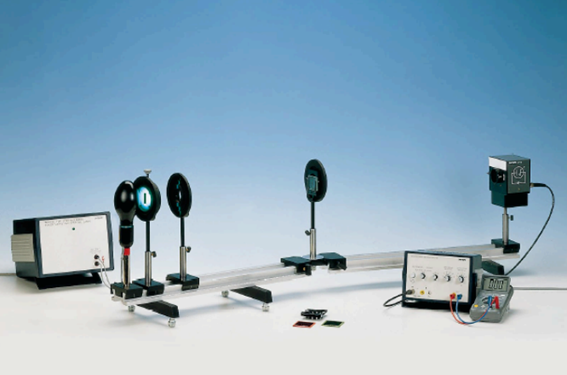
\includegraphics[width=7cm]{Imagem1.png}
    \caption{Montagem do experimento}
    \label{fig:montagem}
\end{figure}

\hspace{1cm} Após a montagem, procede-se ao acionamento da lâmpada de mercúrio, focalizando o feixe luminoso sobre a fotocélula mediante o deslocamento controlado do suporte da lente ao longo do trilho. Deve-se assegurar que a janela da fotocélula permaneça fechada durante o ajuste.

\hspace{1cm} A abertura da fenda deve ser regulada de modo que a imagem luminosa projetada sobre a fotocélula apresente uma largura aproximada de 1 cm, garantindo a incidência uniforme do feixe.

\hspace{1cm} Antes da conexão da fotocélula ao amplificador, configuram-se os instrumentos conforme descrito:

\begin{itemize}
    \item \textbf{Amplificador:}
    \begin{itemize}
        \item Modo de operação: eletrômetro $(R_e > 10^{13}, \Omega)$;
        \item Amplificação: 100;
        \item Constante de tempo: 0.
    \end{itemize}

    \item \textbf{Voltímetro:}

    \begin{itemize}
        \item Escala de 2 V DC.
    \end{itemize}
\end{itemize}

\vspace{.25cm}

\hspace{1cm} O ajuste do zero do amplificador é realizado por meio do botão “0”, mantendo o botão de descarga da fotocélula pressionado, enquanto se observa a leitura do voltímetro.
Uma vez estabilizado o sistema, as medições seguem a seguinte sequência:

\begin{itemize}
    \item Movimentar o trilho para selecionar a faixa monocromática desejada;
    \item Com a janela da fotocélula fechada, verificar o zero do amplificador;
    \item Abrir a janela, aguardar a estabilização da leitura no voltímetro e realizar a medição;
    \item Fechar novamente a janela da fotocélula.
\end{itemize}

\vspace{.25cm}

\hspace{1cm} Durante todo o processo experimental, devem ser observadas as seguintes recomendações de segurança e estabilidade:

\begin{itemize}
    \item Ligar os equipamentos com antecedência mínima de 15 minutos para garantir estabilidade térmica e elétrica;
    \item Evitar desligar a lâmpada de mercúrio, pois o reaquecimento para novo funcionamento requer aproximadamente 10 minutos;
    \item Não tocar no bulbo da lâmpada, cuja temperatura pode ultrapassar 100ºC;
    \item Não olhar diretamente para a fonte de luz, devido à emissão de radiação ultravioleta nociva à visão;
    \item Manter a janela da fotocélula fechada sempre que não estiver sendo efetuada a leitura.
\end{itemize}

% \vspace{.75cm}

\section{RESULTADOS EXPERIMENTAIS}
\hspace{1cm} A partir da execução do procedimento experimental, foram obtidos os seguintes resultados:

\vspace{-.25cm}

\begin{table}[htbp]
    \centering
    \caption{Medições de Tensão em Função da Corrente DC}
    \label{tab:medicoes_tensao}
    \vspace{0.25cm}
    \begin{tabular}{ccc}
        \hline
        \rule{0pt}{3ex}\textbf{Faixa Monocromática} & \textbf{Ângulo} [°] & \textbf{Tensão} [V]\\[5pt]
        \hline
        \rule{0pt}{3ex}Azul 1 & 12 & 0.65 \\
        Azul 2 & 14 & 0.52 \\
        Azul 3 & 16 & 0.51 \\
        Verde & 20 & 0.32 \\
        Laranja & 21 & 0.20 \\[5pt]
        \hline
    \end{tabular}
\end{table}

\vspace{-.25cm}

Partindo do Princípio de Huygens, estabelece-se a seguinte relação fundamental:

\vspace{-.5cm}

\begin{equation*}
    n\,\lambda = d\, \sin{\theta}
\end{equation*}

\vspace{-.15cm}

\hspace{1cm} Em que $\lambda$ representa o comprimento de onda da radiação eletromagnética no vácuo, e $d$ corresponde à distância entre as linhas da rede de difração:

\vspace{-.25cm}

\begin{equation*}
    \lambda = \frac{c}{v}
\end{equation*}

\vspace{-.5cm}

\begin{equation*}
    d = \frac{1}{600}\cdot10^{-3}\,\,[m] = 1.667 \cdot 10^{-6} \,\, [m]
\end{equation*}

\vspace{-.1cm}

\hspace{1cm} Durante o experimento, foram considerados os dados referentes ao primeiro harmônico, sendo utilizada a equação a seguir para o cálculo das frequências de cada faixa espectral:

\vspace{-.25cm}

\begin{equation*}
    v = \frac{c}{d\,\sin{\theta}}\,\,, \quad c = 299'792'458 \,\, \left[\frac{m}{s}\right]
\end{equation*}

\hspace{1cm} Com base nesses valores, foi preenchida a Tabela \ref{tab:medicoes_tensao}. Em seguida foi realizada uma regressão linear e foi construida a figura \ref{fig:grafico} para melhor visualizar os dados recolhidos durante o experimento.

\begin{table}[htbp]
    \centering
    \caption{Medições de Tensão em Função da Corrente DC}
    \label{tab:medicoes_tensao}
    \vspace{0.25cm}
    \begin{tabular}{ccc}
        \hline
        \rule{0pt}{3ex}\textbf{Faixa} & \textbf{Frequência} [Hz] & \textbf{Tensão} [V]\\[5pt]
        \hline
        \rule{0pt}{3ex}Azul 1 & $8.651532\cdot 10^{14}$ & 0.65 \\
        Azul 2 & $7.435271\cdot 10^{14}$ & 0.52 \\
        Azul 3 & $6.525802\cdot 10^{14}$ & 0.51 \\
        Verde & $5.259207\cdot 10^{14}$ & 0.32 \\
        Laranja & $5.019296\cdot 10^{14}$ & 0.20 \\[5pt]
        \hline
    \end{tabular}
\end{table}

\begin{figure}[h]
    \centering
    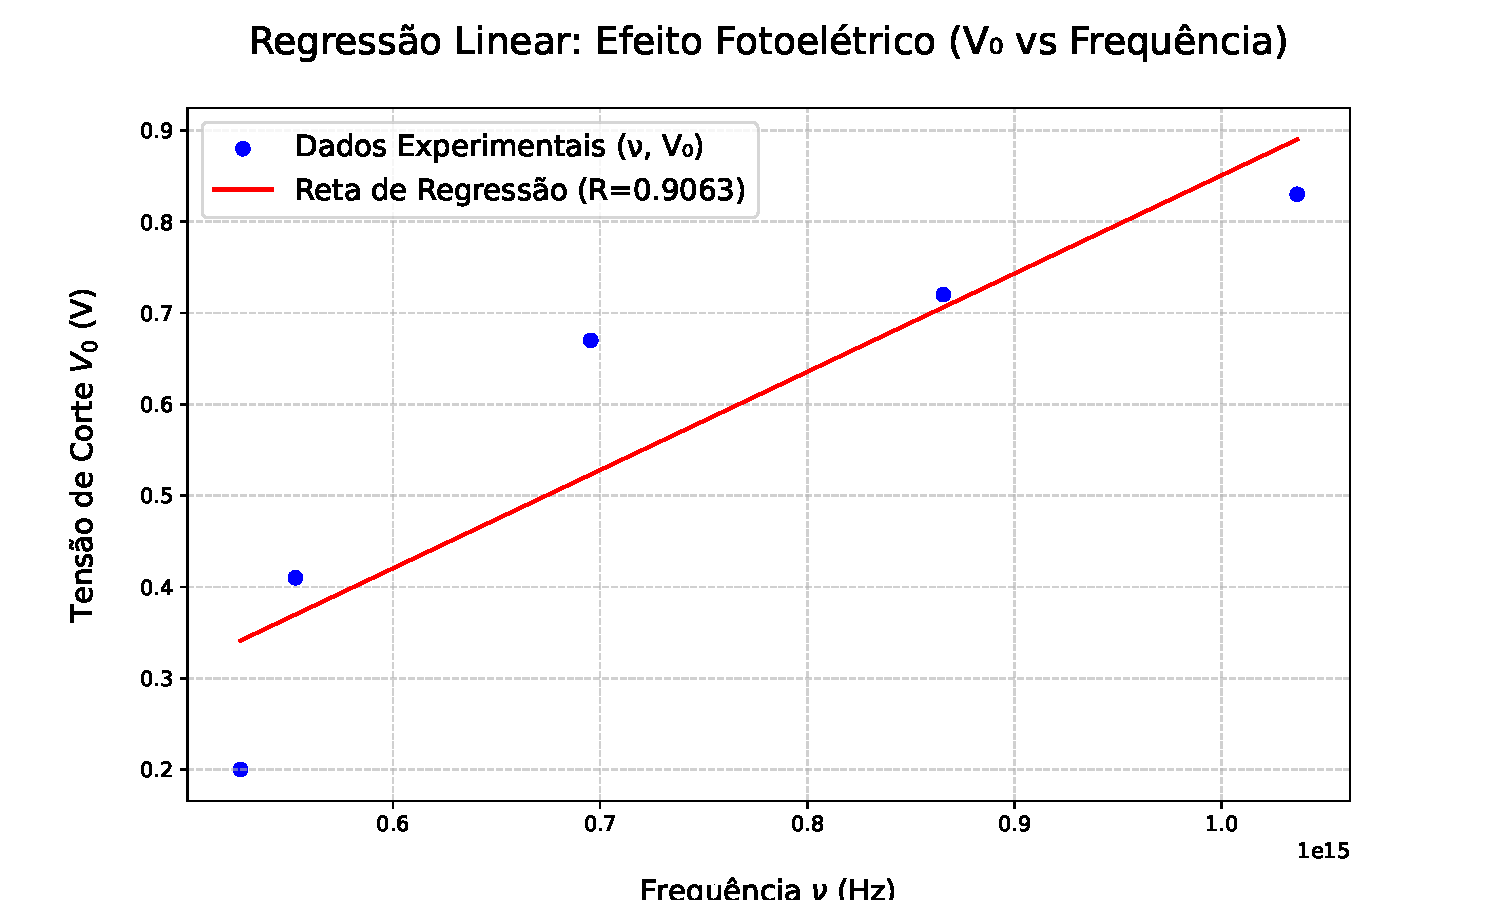
\includegraphics[width=8.5cm]{efeito_fotoeletrico_regressao.pdf}
    \caption{Resultados distribuidos graficamente}
    \label{fig:grafico}
\end{figure}

\noindent Dessa análise obteve-se a equação experimental:

{\Huge \color{red} *VER* EQUAÇÕES}

{\color{red} Não sei da onde veio esses valores e essas equações.}

\vspace{12cm}

{
    \color{red}

\begin{equation*}
    e^-\cdot V_0 = 8.651532\cdot 10^{14} \cdot h - 4.76700997 \cdot 10^{-20}
\end{equation*}

Sejam $ e^- = 1.6\cdot10^{-19}$ e $V_0 = 0.65$;
\begin{equation*}
    (1.6\cdot10^{-19})\cdot V_0 = 8.651532\cdot 10^{14} \cdot h - 4.76700997 \cdot 10^{-20}
\end{equation*}

\begin{equation*}
    15.16700997 \cdot 10^{-20} = 8.651532\cdot 10^{14} \cdot h
\end{equation*}

\begin{equation*}
    h = \frac{15.16700997}{8.651532} = 1.7531010658
\end{equation*}

}

========================

{
    \color{red}

\begin{equation*}
    e^-\cdot V_0 = 8.651532\cdot 10^{14} \cdot h - 4.76700997 \cdot 10^{-20}
\end{equation*}

Sejam $ e^- = 1.6\cdot10^{-19}$ e $V_0 = 0.65$;
\begin{equation*}
    (1.6\cdot10^{-19})\cdot V_0 = 8.651532\cdot 10^{14} \cdot h - 4.76700997 \cdot 10^{-20}
\end{equation*}

\begin{equation*}
    15.16700997 \cdot 10^{-20} = 8.651532\cdot 10^{14} \cdot h
\end{equation*}

\begin{equation*}
    h = \frac{15.16700997}{8.651532} = 1.7531010658
\end{equation*}

}

\begin{equation*}
    V_0 = 8.651532\cdot 10^{14} \cdot v - 4.76700997 \cdot 10^{-20}
\end{equation*}

\hspace{1cm} Multiplicando-se a equação acima pela carga elementar do elétron $(e = 1.6 \cdot 10^{-19} \,\, [C])$, chega-se a:

\begin{equation*}
    K_{\max} = eV_0 = 1.7211 \cdot 10^{-34}\,v - 0.225054003\,e
\end{equation*}

\hspace{1cm} Considerando a expressão $K_{\max} = h\,v - \Phi\,$, determinam-se os valores da constante de Planck e da função trabalho do material:

\begin{equation*}
    h = 1.7211\cdot 10^{-34} \,\, [J\,.\,s]
\end{equation*}

\begin{equation*}
    \Phi = 0.225054003\,e
\end{equation*}

\noindent Por fim, a frequência de corte é obtida quando $K_{\max} = 0$:

\begin{equation*}
    v_0 = 2.09218 \cdot 10^{14} \,\, Hz
\end{equation*}

% \vspace{.75cm}

\section{ANALISE DOS RESULTADOS EXPERIMENTAIS}

\noindent\textit{A. Sobre o valor da constante de Planck e potencial de
retardo}

\noindent O valor teórico da constante de Planck é aproximadamente:

\vspace{-.3cm}

\begin{equation*}
    h = 6.63 \cdot 10^{-34} \,\, [J\,.\,s]
\end{equation*}

\vspace{-.22cm}

\hspace{1cm} Ao comparar esse valor teórico com o resultado obtido experimentalmente, observa-se uma discrepância atribuível à sensibilidade da fotocélula e à dificuldade de isolar radiações de frequência única no sistema óptico. Apesar dessas limitações, o valor obtido mantém-se dentro da mesma ordem de grandeza esperada, validando a metodologia empregada.

\hspace{1cm} Além disso, nota-se que materiais com maior potencial de retardo tendem a gerar resultados mais precisos, pois a diferença de potencial mais elevada permite a identificação mais nítida do ponto de corte fotoelétrico.

\noindent\textit{B. Sobre a função trabalho e frequência de corte}

\hspace{1cm} A função trabalho representa a energia mínima necessária para a ejeção de um elétron da superfície do material. Assim, ela constitui um parâmetro característico que permite identificar o material constitutivo da fotocélula.

\hspace{1cm} A frequência de corte está diretamente relacionada à função trabalho, sendo definida como a frequência mínima do fóton capaz de causar a emissão eletrônica.

\hspace{1cm} A física clássica não é capaz de explicar adequadamente o efeito fotoelétrico, pois este fenômeno exige a consideração da natureza dual da luz, que se manifesta tanto como onda quanto como partícula.

\noindent\textit{C. Sobre a célula fotoelétrica e a relação de absorção de
fótons na frequência de corte e a tensão medida.}

\hspace{1cm} A luz incidente, ao atravessar uma janela de quartzo, incide sobre uma placa metálica, provocando a emissão de elétrons (fotoelétrons). Estes são coletados por um eletrodo metálico devido à diferença de potencial existente entre os dois condutores.
Quando a tensão aplicada é suficientemente alta, todos os elétrons emitidos são coletados, resultando na saturação da corrente fotoelétrica.

\hspace{1cm} A frequência de corte corresponde ao limiar abaixo do qual o efeito fotoelétrico não ocorre. Quando a radiação incidente possui frequência superior à de corte, cada fóton absorvido transfere sua energia a um elétron, causando sua ejeção imediata e originando uma corrente fotoelétrica mensurável.

% \vspace{.75cm}

\section{Conclusão}

\hspace{1cm} O experimento permitiu a observação direta do efeito fotoelétrico e a comprovação empírica dos conceitos fundamentais da física quântica.

\hspace{1cm} Verificou-se que a energia dos elétrons emitidos pela fotocélula depende exclusivamente da frequência da luz incidente, e não de sua intensidade, evidenciando o comportamento corpuscular da radiação.

\hspace{1cm} A determinação da frequência de corte e da função trabalho demonstrou a coerência entre os resultados obtidos e a teoria proposta por Einstein.

\hspace{1cm} Conclui-se, portanto, que as características observadas só podem ser explicadas considerando a dualidade da luz, que se propaga como onda, mas interage com a matéria como partícula — o fóton.

% \vfil
\section{REFERENCIAS BIBLIOGRAFICAS}

{\small
\begin{enumerate}

    \item CESCHIN, Artemis M. Apostila de materiais eletricos e magneticos.

    \item REZENDE, Sergio M. Materiais e Dispositivos Eletrônicos. 2ª ed. São Paulo: Editora Livraria da Física, 2004.

    \item HAYT, W. H. Jr. Eletromagnetismo. 6ª ed. Rio de Janeiro: LTC, 1995.
    
\end{enumerate}
}

\end{document}